\documentclass{article}
\usepackage[utf8]{inputenc}
\usepackage{amsmath}
\usepackage{amssymb}
\usepackage{amsthm}
\renewcommand{\qedsymbol}{\ensuremath{\blacksquare}}
\renewcommand{\thesubsection}{\thesection.\alph{subsection}}
\usepackage[a4paper, total={6in, 8in}]{geometry}
\usepackage[pdftex]{graphicx}
\usepackage[english]{babel}
\usepackage{float}
\usepackage{comment}
\usepackage{float,graphicx}
\usepackage{afterpage}
\usepackage{xcolor}
\usepackage{caption}
\usepackage{subcaption}
\usepackage{placeins}

\title{TFY4240 Assignment Problem 1}
\date{Mars 2021}
\author{Jostein Kløgetvedt}
\begin{document}

\maketitle


\section*{Introduction}
In this exercise we will try to determine the electric potential and the corresponding electric field in a long, square and hollow tube. Since the tube is long in one of the directions we neglect the boundaries and simulate the potential inside the tube with a 2-dimensional potential $V(x,y)$. 
The potential is given by Laplace's equation
\begin{equation}
\label{Laplace}
    \nabla ^2V =  \frac{\partial^2V}{\partial x^2} + \frac{\partial^2V}{\partial y^2} = 0.
\end{equation}
The boundary conditions on each side of the wall inside the tube are 
\begin{equation}
    \begin{split}
        V(0,y) &= 0 \\
        V(L,y) &= 0 \\
        V(x,0) &=0 \\
        V(x,L) &= V_0(x), 
    \end{split}
\end{equation}
where $L$ is the dimension of the square tube in $x$- and $y$-direction, and $V_0(x)$ is a function not yet specified.

We will start by converting the equation \eqref{Laplace} into a dimensionless equation. Afterwards we will find a general solution of the potential using the method of separation of variables. We are going to consider three types of boundary functions $V_0(x)$ where we for each case show convergence of the numerical solution, the potential across the tube and the corresponding electric field. To find the electric field we use the formula $\boldsymbol{E}(x,y)= - \nabla V(x,y)$. 

\section*{Theory}
\subsection*{Dimensionless equation}

By introducing the dimensionless parameters $\xi = x/L$, $\eta = y/L$ and $U = V/V_c$ we can make the equation dimensionless, 
\begin{equation}
\begin{split}
    V_{xx} + V_{yy} = 0 &\Rightarrow V_cU_{xx} + V_cU_{yy} = 0 \\
    \Rightarrow U_{xx} + U_{yy} = 0 &\Rightarrow \frac{U_{\xi\xi}}{L} + \frac{U_{\eta\eta}}{L} = 0 \\ &\Rightarrow U_{\xi\xi} + U_{\eta\eta} = 0.
\end{split}  
\end{equation}

Now with $0 \leq \xi \leq 1$ and $0 \leq \eta \leq 1$ the new boundary conditions becomes 
\begin{equation}
    \begin{split}
        U(0,\eta) &= 0 \\
        U(1,\eta) &= 0 \\
        U(\xi,0) &=0 \\
        U(\xi,1) &= U_0(\xi).
    \end{split}
\end{equation}

From here on we are only going to look at the dimensionless equation but where we change the name of variables back again to $\xi \rightarrow x$, $\eta \rightarrow y$ and $U \rightarrow V$ and remember that $0 \leq x,y \leq 1$. This also applies for the plots shown below. 

\subsection*{General solution to the boundary value problem}
As stated in the introduction we shall solve the Laplace equation with the method of separation of variables and formulate the solution in a Fourier series expansion. The coming derivation is based on an example from chapter three in the the book \emph{Introduction to electrodynamics} \cite{Griffiths}. Assuming the potential can be written as $V(x,y)=X(x)Y(y)$ we insert it in equation \eqref{Laplace} and find
\begin{equation}
    \frac{X''(x)}{X(x)} = - \frac{Y''(y)}{Y(y)}.
\end{equation}
Now since the left hand side only depends on $x$ and the right hand side only depends on $y$ both terms must be equal to a constant. If the constant is zero we will get a linear solution for both $X(x)$ and $Y(y)$ and combining the boundary conditions we are left with only a trivial solution where the potential is zero, which is a solution we are not interested in.

Now checking for a solution with a positive constant we call $k^2$ we find
\begin{equation}
    X''(x) = k^2X(x) \Rightarrow X(x) = A e^{k x}+Be^{-k x}.
\end{equation}
Using the boundary conditions to determine the coefficients we find
\begin{equation}
    V(0,y) = X(0)Y(y) = 0 \Rightarrow X(0) = 0 \Rightarrow A = -B,
\end{equation}
and for the other boundary 
\begin{equation}
\begin{split}
    V(1,y) = X(1)Y(y) = 0 \rightarrow X(1)=0 \rightarrow A e^{k} + Be^{-k}=0 \rightarrow A(e^k-e^{-k})=0.
\end{split}
\end{equation}
The equation is fulfilled if either $A=0$ or $k=0$, where in both cases we only get a trivial solution.

Now checking the final option where the constant is negative, $-k^2$. Here we get a harmonic solution for $X(x)$ and an exponential for $Y(y)$, namely
\begin{equation}
    X(x) = A\sin{k x} + B\cos{k x} \text{,}\hspace{3mm} Y(y)=Ce^{k y}+D e^{-k y}.
\end{equation}
Again we use the boundary conditions to determine the coefficients
\begin{equation}
\begin{split}
    X(0)&=0 \Rightarrow B=0 \\
    Y(0)&=0 \Rightarrow C=-D \\
    X(1)&=0 \Rightarrow A\sin{(k)}=0 \Rightarrow k_n=n\pi \text{,  } n=\dots {-1},0,1,\dots
\end{split}
\end{equation}
Now we can combine the two functions $X$ and $Y$ to find the potential
\begin{equation}
    V_n(x,y) =  A' \sin{(n\pi x)}(e^{n\pi y}-e^{-n\pi y}) = A'' \sin{(n\pi x)} \sinh{(n\pi y)},
\end{equation}
where $A'$ and $A''$ just are new constants merged from old ones. Using superposition we find a general solution for the potential 
\begin{equation}
\label{General solution}
    V(x,y) = \sum_{n=1}^{\infty} D_n \sin{(n\pi x)} \sinh{(n \pi y)},
\end{equation}
where we call the coefficient for each term $D_n$ and we only sum from $n=1$ and upwards because the terms below $n=0$ will not give any new solutions. To determine the coefficients we use the so called Fourier's trick where we multiply the last boundary equation with a sine term for then to integrate over the boundary and use the sine-orthogonality to determine every $D_n$.

\begin{equation}
\begin{split}
\label{coefficients}
&V(x,1) = V_0(x)  = \sum_{n=1}^{\infty} D_n \sin{(n\pi x)} \sinh{(n \pi)} \\
\Rightarrow &\int_0^1 V_0(x) \sin{(m\pi x)} dx = \sum_{n=1}^{\infty} D_n \sinh{(n\pi)}\int_0^1 \sin{(m\pi x)} \sin{(n\pi x)} dx \\
\Rightarrow &D_m = \frac{2}{\sinh{(m\pi)}} \int_0^1 V_0(x) \sin{(m\pi x)}dx.
\end{split}
\end{equation}

With a given boundary function $V_0(x)$ we can now determine the potential explicitly in a Fourier series. The Fourier series can easily be calculated numerically where we choose the accuracy with the order we sum the series up to and for each term use an appropriate integration method to find the coefficient.  


\section*{Results}
We shall now consider different types of boundary functions $V_0(x)$ where we calculate the numerical solution for the electric potential and the corresponding electric field and investigate how fast the solution convergences. 

\subsection*{Sine boundary potential}
With our dimensionless parameters we choose a boundary function on the form $V_0(x)=\sin{(4\pi x)}$. With this rather simple potential we can calculate the potential analytically by using the formula \eqref{coefficients} to determine the coefficients.
\begin{equation}
\begin{split}
    D_n &= \frac{2}{\sinh{(n\pi)}} \int_0^1 \sin{(4\pi x)}\sin{(n\pi x)}dx = \frac{2}{\sinh{(n\pi)}} \frac{1}{2} \delta_{4n} \\ &\Rightarrow D_4 = \frac{1}{\sinh{(4\pi)}} \text{,} \hspace{3mm} D_n = 0 \text{ for} \hspace{2mm} n \neq 4.
\end{split}
\end{equation}
The potential then becomes 
\begin{equation}
    V(x,y) = \frac{\sin{(4\pi x)} \sinh{(4\pi y)}}{\sinh{(4\pi)}}.
\end{equation}

With this boundary function we only need to sum the Fourier series to the fourth term and we get the exact solution.

In figure \ref{fig: V_sinepot3D&contour} we can see a 3D plot and a contour plot of the potential in the tube. In the figures \ref{fig:V(x,1)_sinepot} and \ref{fig:other_bond_sinepot} we can see how the numerical solution of $V(x,y)$ fulfill the boundary conditions. Figure \ref{fig: Efield_sinepot} shows how the electric field changes both with magnitude and direction using arrows as a form of representation.

\begin{figure}[!htb]
     \centering
     \begin{subfigure}[b]{0.4\textwidth}
         \centering
         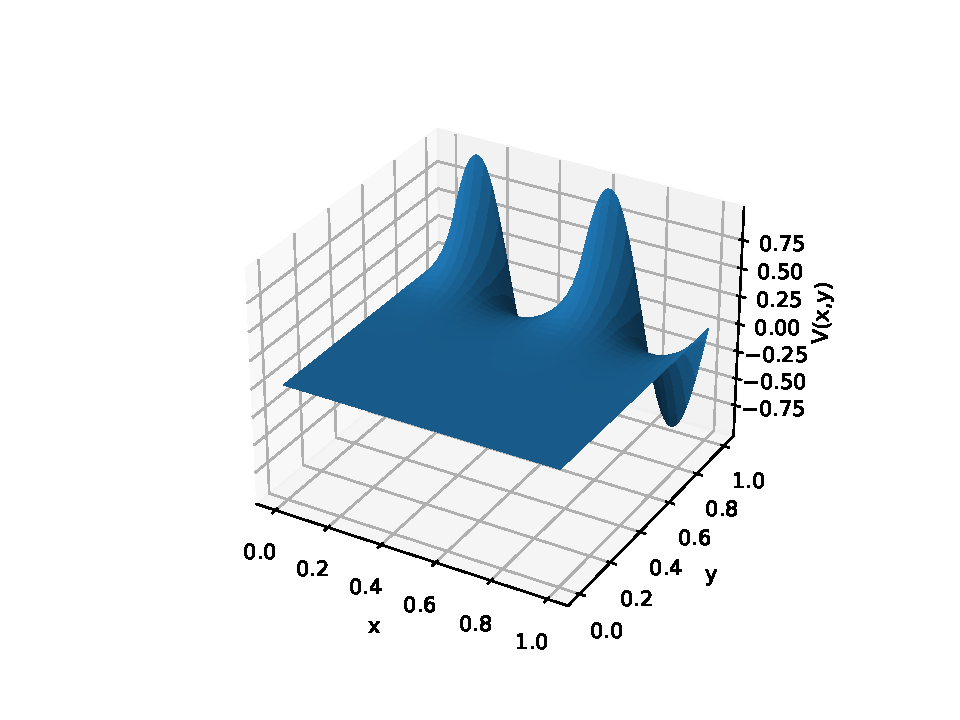
\includegraphics[width=1.6\linewidth]{V_sinepot3D.pdf}
     \end{subfigure}
    %\hfill
    \hspace{6em}
     \begin{subfigure}[b]{0.4\textwidth}
         \centering
         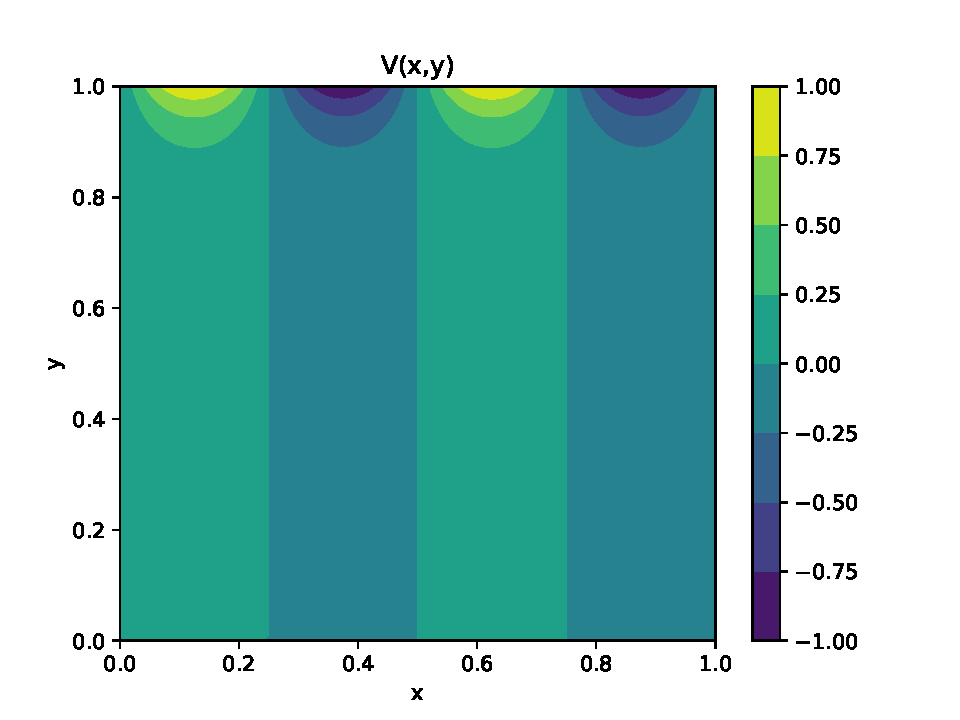
\includegraphics[width=1.4\linewidth]{V_sinepot_contourf.pdf}
     \end{subfigure}
    \caption{3D and contour plot of $V(x,y)$.}
    \label{fig: V_sinepot3D&contour}
\end{figure}

\begin{figure}[!htb]
\centering
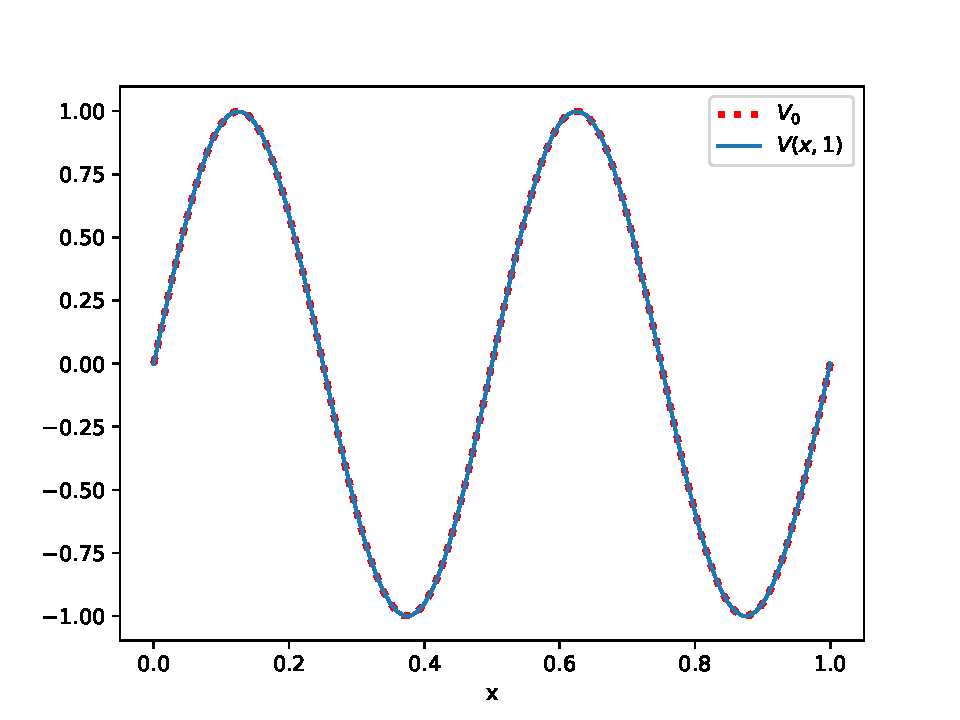
\includegraphics[width=10cm]{V(x,1)_sinepot.pdf}{}
\caption{Plot of $V(x,1)$ and $V_0(x)$ to check if boundary condition is fulfilled.}
\label{fig:V(x,1)_sinepot}
\end{figure}


\begin{figure}[!htb]
\centering
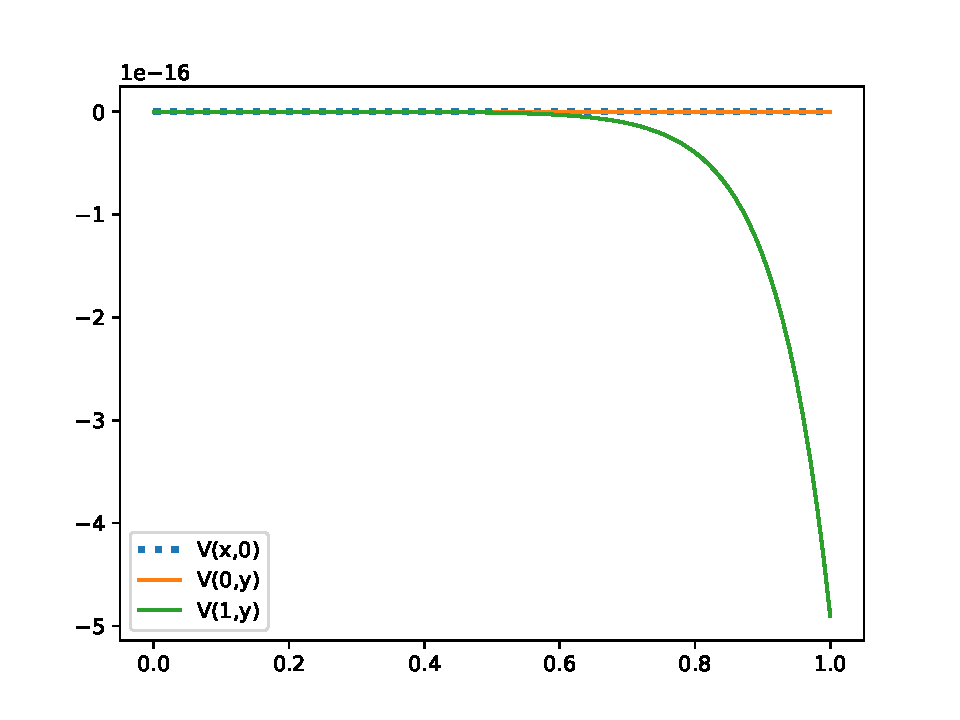
\includegraphics[width=10cm]{boundaries_sinepot.pdf}{}
\caption{Plot of $V(x,y)$ at the boundaries where $x=0,L$ and $y=0$. The bottom axis is meant to represent both $x$ and $y$ depending on which potential we are looking at.}
\label{fig:other_bond_sinepot}
\end{figure}

\begin{figure}[!htbp]
\centering
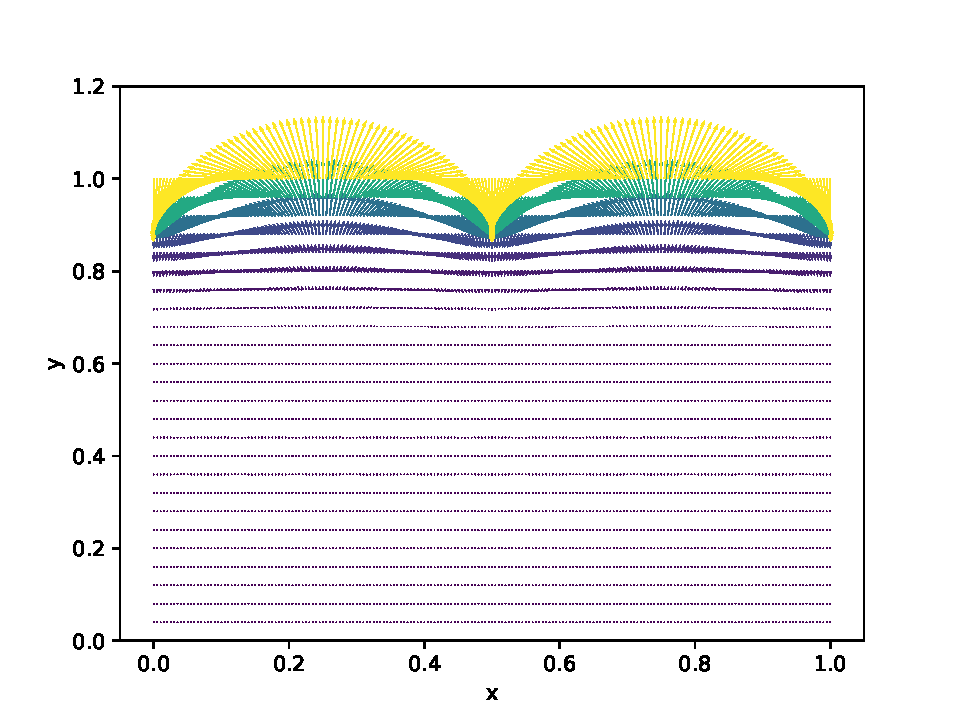
\includegraphics[width=12cm]{Efield_sine.pdf}{}
\caption{Plot of the electric field $\boldsymbol{E}(x,y)$.}
\label{fig: Efield_sinepot}
\end{figure}
\FloatBarrier

\subsection*{Quadratic boundary potential}
Here we will look at the boundary function $V_0(x)=1 - 16(x-\frac{1}{2})^4$. The function fulfills the other requirements, namely that $V_0(x=0)=0$ and $V_0(x=1)=0$. 

We will investigate how the numerical solution converge towards the boundary function and use that as an estimate for what order the potential is accurate enough on the whole square. From figure \ref{fig: V(x,1)_quadpot} we can see that the numerical solution at the boundary $y=1$ converges towards $V_0(x)$ very fast. When we sum up the Fourier series to order $n=7$ we struggle to see a difference between the two of them.
\begin{figure}[!htb]
\centering
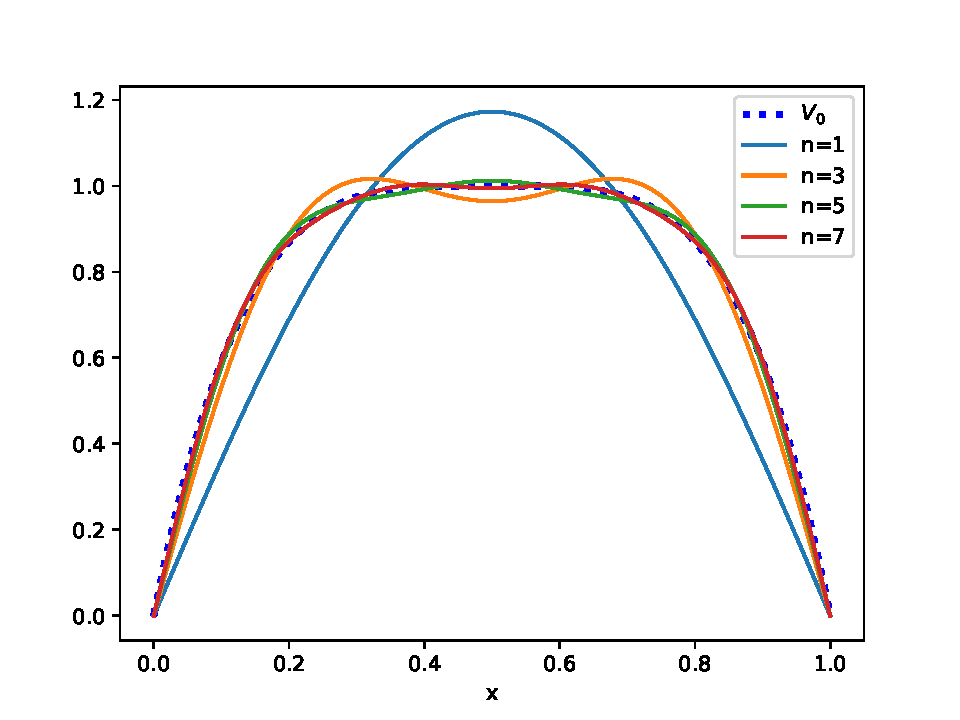
\includegraphics[width=10cm]{V(x,1)_quadpot.pdf}{}
\caption{Plot of $V_0(x)$ and $V(x,1)$ for different orders $n=1,3,5,7$.}
\label{fig: V(x,1)_quadpot}
\end{figure}

To give an estimate of how many orders we need to find a satisfying solution of the potential we calculate the relative error of $V(x,1)$ compared to $V_0(x)$ as a function of the order we sum up to. The relative error is in this case the discrete Frobenius norm and is on the form $e_r = \frac{||V(x,1)-V_0(x)||}{||V_0(x)||}$. From plot \ref{fig: error_quadpot} we can see that the error only decreases every other order. That is because all the terms in the Fourier series with even $n$ are asymmetric with respect to $x=\frac{1}{2}$ and will not contribute to the symmetric boundary function. To get a satisfying potential we might want a relative error below $10^{-2}$, and to get that we can use an order of $n=10$ and higher. 

\begin{figure}[!htb]
\centering
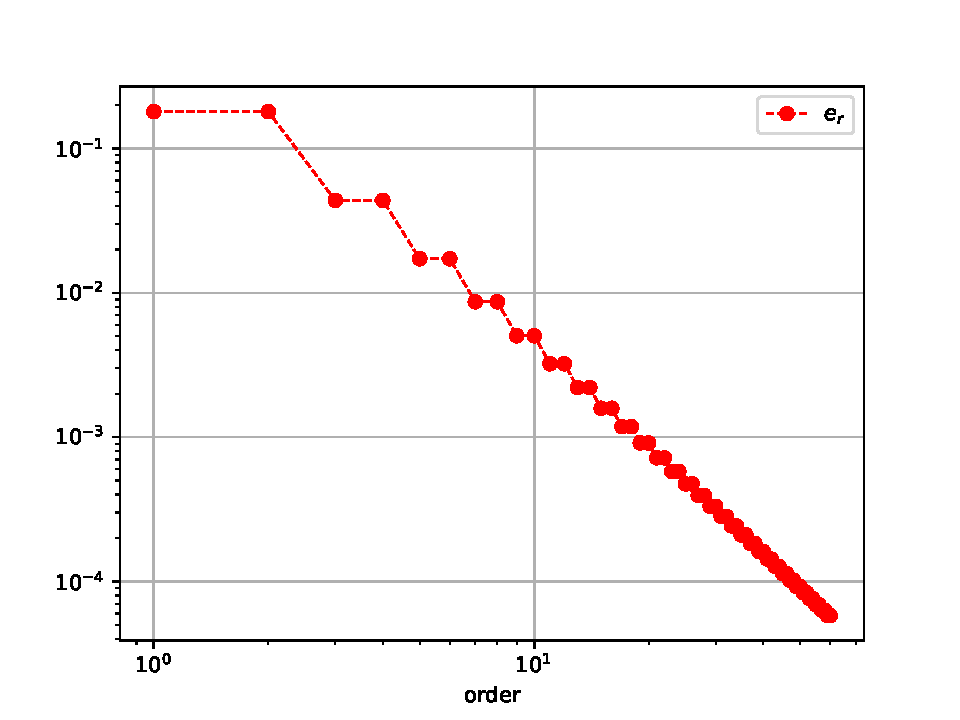
\includegraphics[width=10cm]{error_quadpot.pdf}{}
\caption{Relative error of $V(x,1)$ compared to the desired result $V_0(x)$. Plotted as a function of orders from 1 to 60. }
\label{fig: error_quadpot}
\end{figure}

From the convergence analysis we choose the order $n=10$ to be sufficient and plot the potential at the whole tube and check whether the potential fulfills the boundary condition at the three other walls. Figure \ref{fig: V_quadpot_contourf} shows a contour plot of the potential $V(x,y)$ and figure \ref{fig: boundaries_quadpot} shows that the potential is indeed zero at the other three walls. The reason why $V(1,y)$ is not exactly zero is due to the machine precision.

The corresponding electric field $\boldsymbol{E}(x,y)$ is shown in figure \ref{fig: Efield_quadpot} where we have shown both an arrow representation and a contour plot of the absolute value of the electric field. 

\begin{figure}[!htb]
\centering
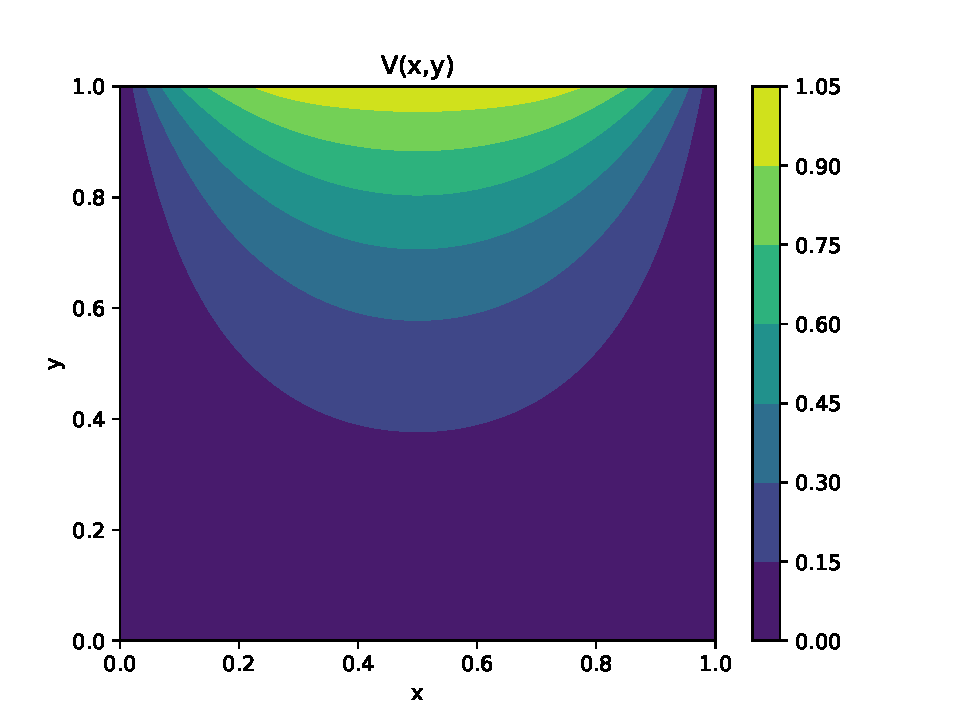
\includegraphics[width=10cm]{V_quadpot_contourf.pdf}{}
\caption{Contour plot of $V(x,y)$.}
\label{fig: V_quadpot_contourf}
\end{figure}

\begin{figure}[!htb]
\centering
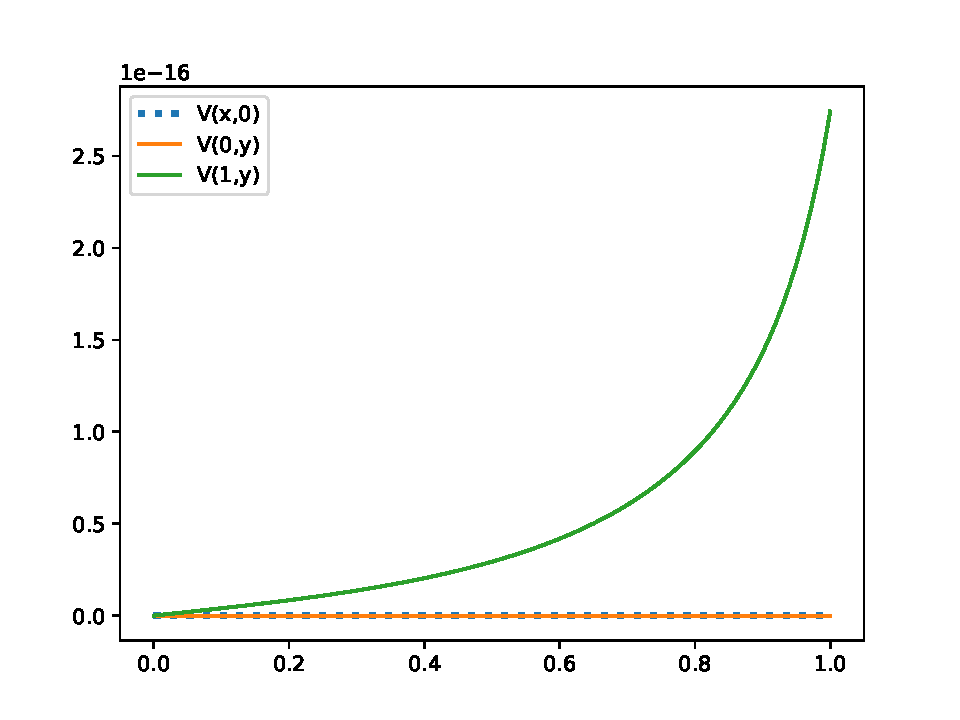
\includegraphics[width=10cm]{boundaries_quadpot.pdf}{}
\caption{Plot of $V(x,y)$ at the boundaries where $x=0,L$ and $y=0$. The bottom axis is meant to represent both $x$ and $y$ depending on which potential we are looking at. }
\label{fig: boundaries_quadpot}
\end{figure}

\begin{figure}[!htbp]
     \centering
     \begin{subfigure}[b]{0.4\textwidth}
         \centering
         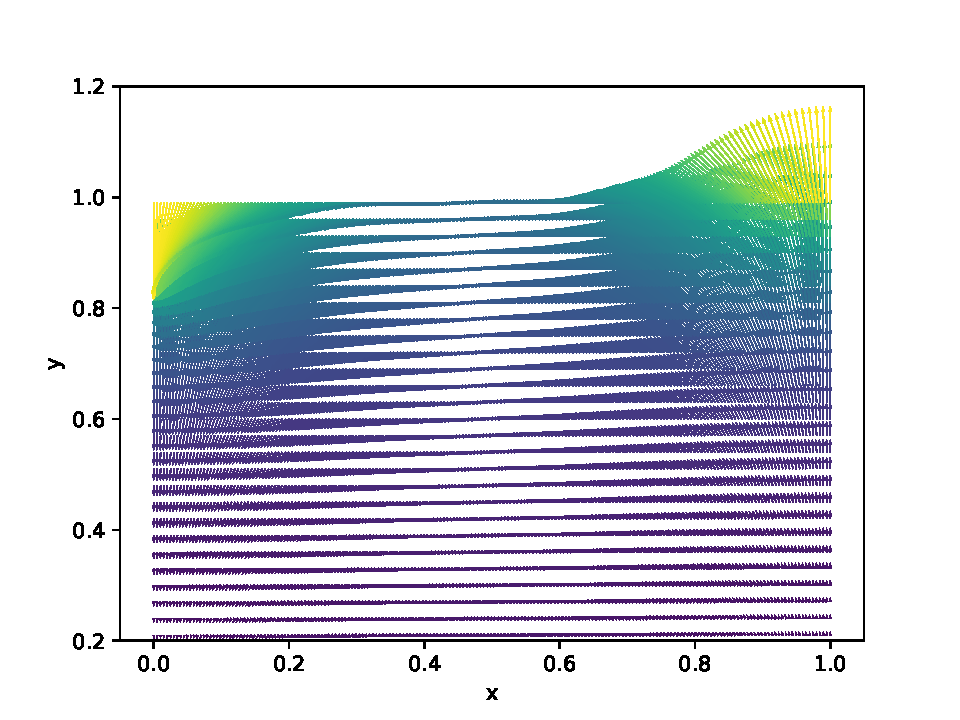
\includegraphics[width=1.5\linewidth]{Efield_quadpot.pdf}
         \caption{$\boldsymbol{E}(x,y)$}
     \end{subfigure}
    %\hfill
    \hspace{6em}
     \begin{subfigure}[b]{0.4\textwidth}
         \centering
         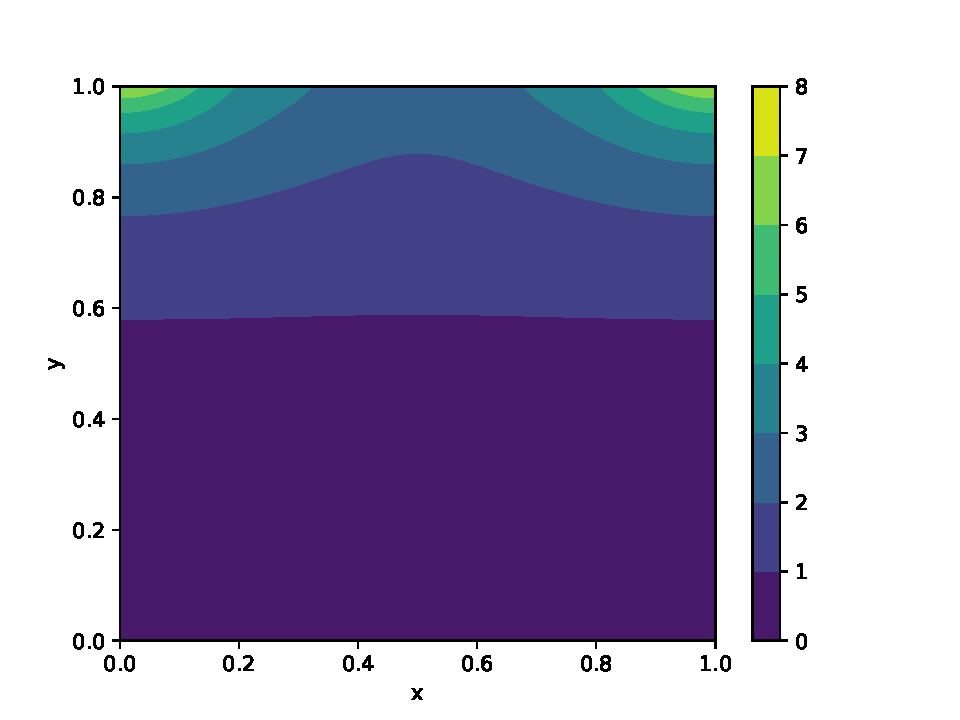
\includegraphics[width=1.5\linewidth]{Efield_contour_quad.pdf}
         \caption{$|\boldsymbol{E}(x,y)|$}
     \end{subfigure}
    \caption{Plot of $\boldsymbol{E}(x,y)$ and contour plot of $|\boldsymbol{E}(x,y)|$.}
    \label{fig: Efield_quadpot}
\end{figure}
\FloatBarrier

\subsection*{Heaviside step function as boundary potential}
We will here use a boundary potential on the form $V_0(x) = \theta(x-\frac{1}{2})\theta(\frac{3}{4}-x)$ where $\theta(x)$ is the Heaviside step function. 

In the same manner as earlier we first show how the potential at the boundary $y=1$ converges towards the Heaviside step function boundary potential $V_0(x)$. This can be seen in figure \ref{fig: V(x,1)_Heavisidepot}. Due to the discontinuity in the boundary function it takes a very long time, perhaps even infinite time, to converge. The reason for this is because we use a series of continuous functions to approximate a discontinuous function. This is commonly known as Gibbs phenomenon. 

The relative error of $V(x,1)$ compared to $V_0(x)$ is shown in figure \ref{fig: error_Heavisidepot}. The error converges very slowly as mentioned earlier. It's hard to get a relative error less than $10^{-2}$ so we will settle for a relative order around $10^{-1}$ by using a order of $n=100$ we sum up to in the Fourier series. 

In figure \ref{fig: V_Heaviside} we see the potential at the whole tube as a 3D-plot and as a contour plot. From figure \ref{fig: boundaries_Heaviside} we can see that the potential $V(x,y)$ fulfills the other boundary conditions by being zero at the other three walls. The corresponding electric field $\boldsymbol{E}(x,y)$ is shown in figure \ref{fig: Efield_Heaviside}.

\begin{figure}[!htb]
\centering
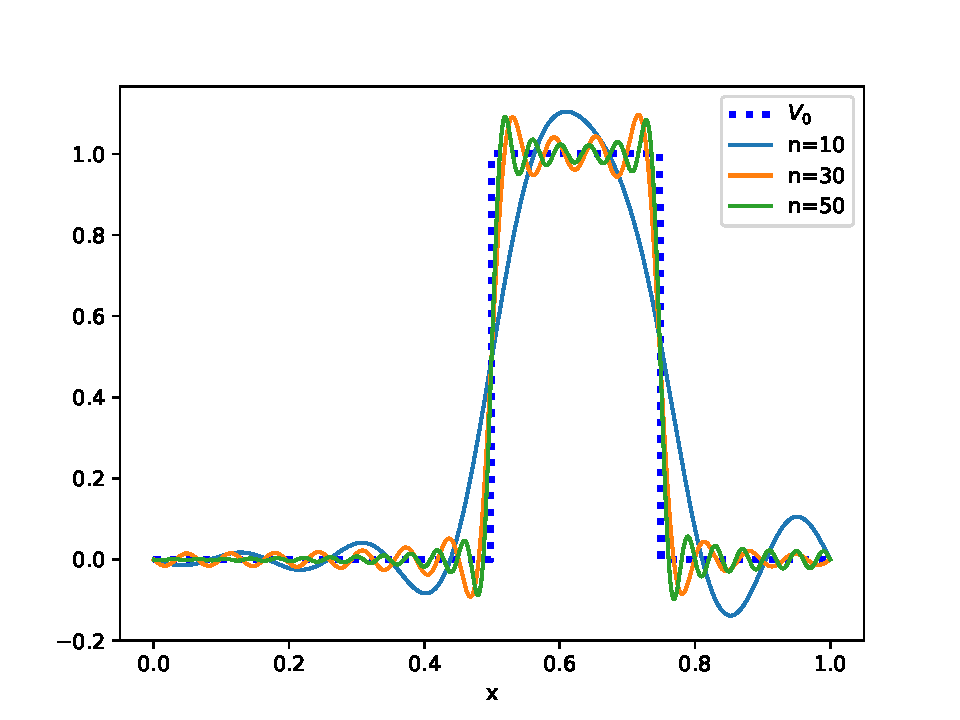
\includegraphics[width=10cm]{V(x,1)_Heavisidepot.pdf}{}
\caption{Plot of $V_0(x)$ and $V(x,1)$ for different orders $n=10,30,50$. }
\label{fig: V(x,1)_Heavisidepot}
\end{figure}

\begin{figure}[!htb]
\centering
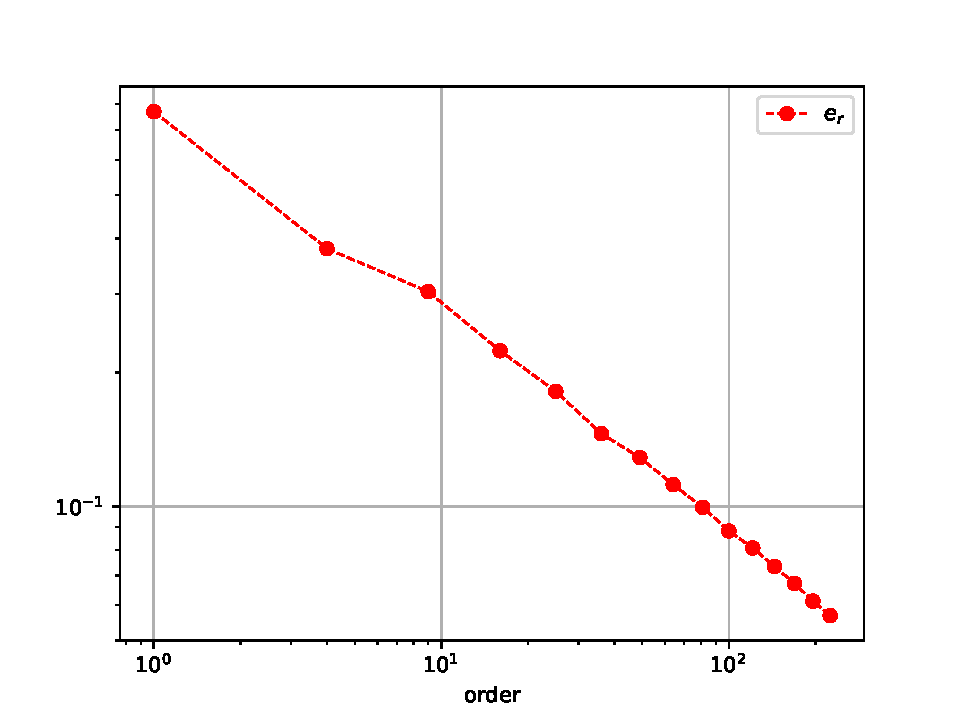
\includegraphics[width=10cm]{error_Heavisidepot.pdf}{}
\caption{Relative error of $V(x,1)$ compared to the desired result $V_0(x)$. Plotted as a function of orders. }
\label{fig: error_Heavisidepot}
\end{figure}

\begin{figure}[!htb]
     \centering
     \begin{subfigure}[b]{0.4\textwidth}
         \centering
         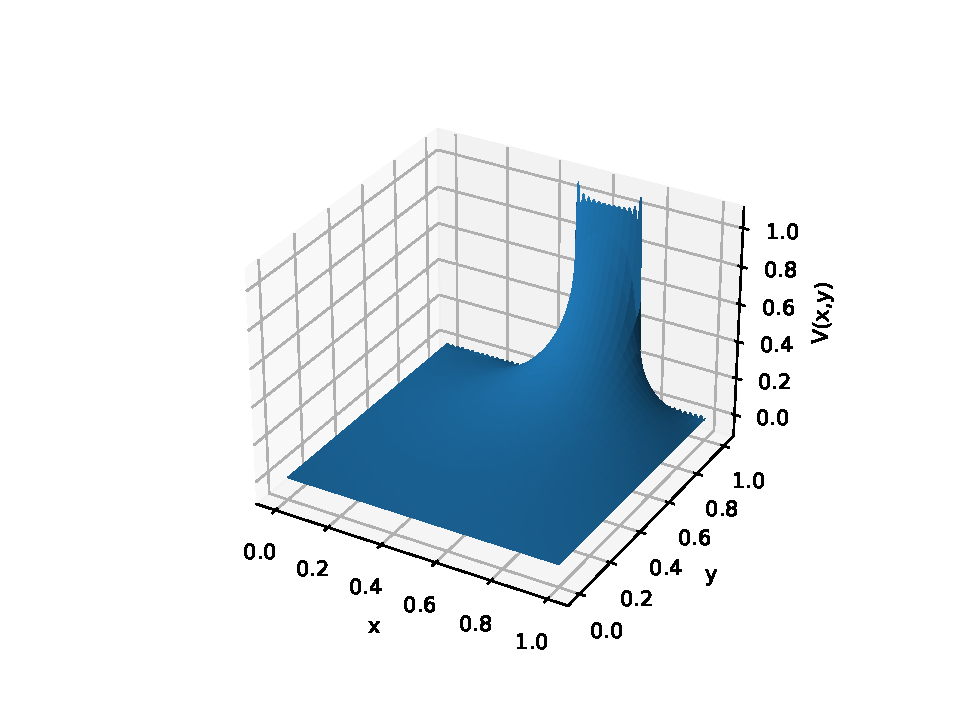
\includegraphics[width=1.6\linewidth]{V_Heaviside3D.pdf}
     \end{subfigure}
    %\hfill
    \hspace{6em}
     \begin{subfigure}[b]{0.4\textwidth}
         \centering
         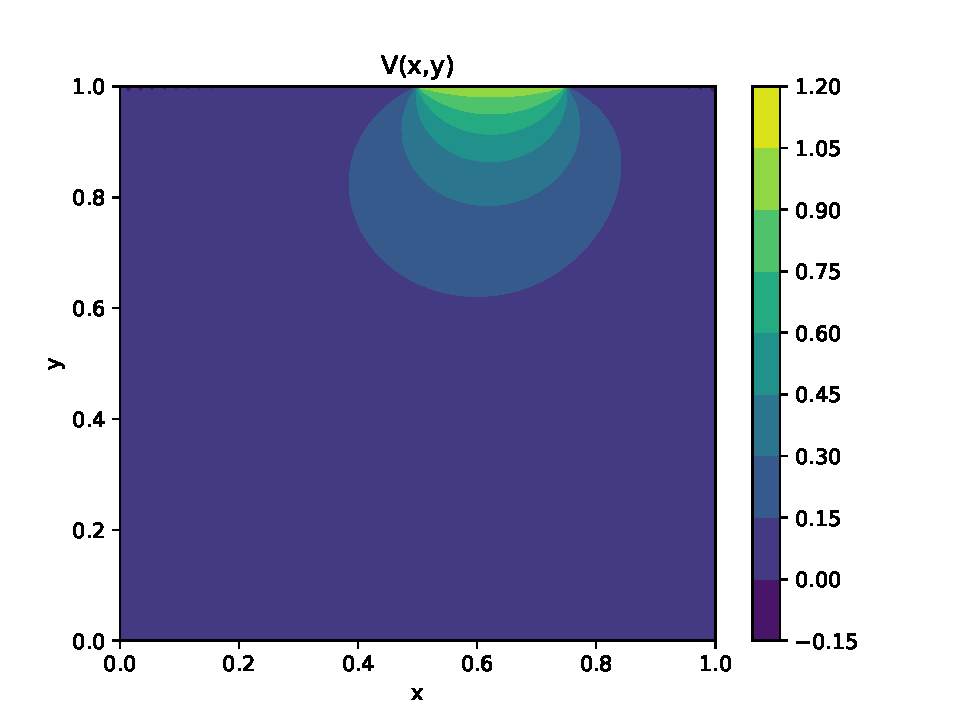
\includegraphics[width=1.4\linewidth]{V_Heaviside_contourf.pdf}
     \end{subfigure}
    \caption{3D and contour plot of $V(x,y)$.}
    \label{fig: V_Heaviside}
\end{figure}

\begin{figure}[!htb]
\centering
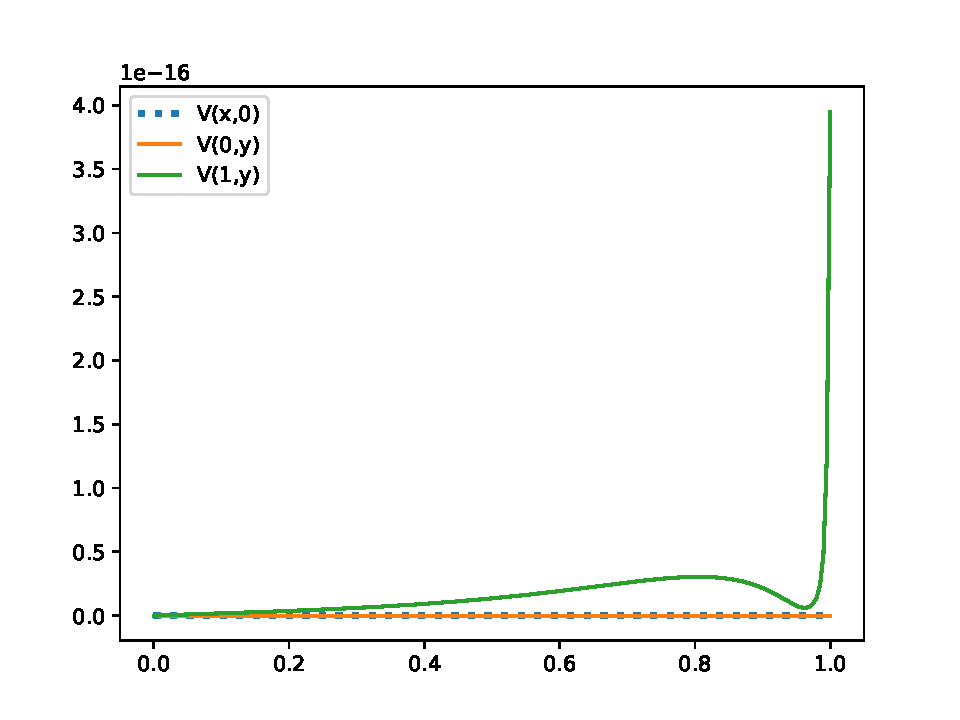
\includegraphics[width=10cm]{boundaries_Heaviside.pdf}{}
\caption{Plot of $V(x,y)$ at the boundaries where $x=0,L$ and $y=0$. The bottom axis is meant to represent both $x$ and $y$ depending on which potential we are looking at.}
\label{fig: boundaries_Heaviside}
\end{figure}

\begin{figure}[!htbp]
\centering
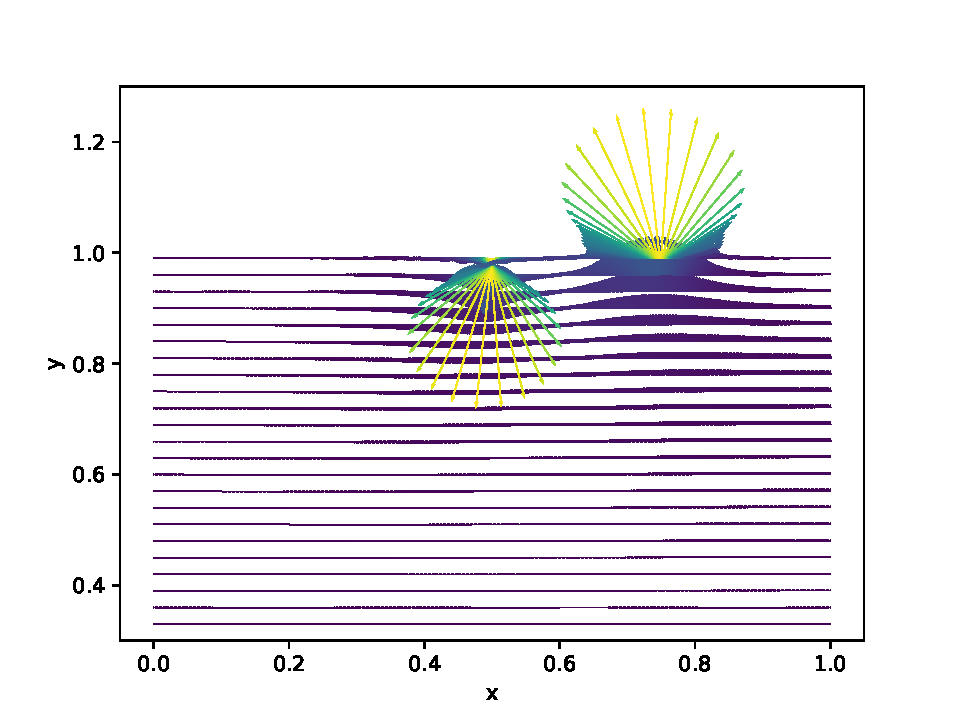
\includegraphics[width=12cm]{Efield_Heaviside.pdf}{}
\caption{Plot of the electric field $\boldsymbol{E}(x,y)$.}
\label{fig: Efield_Heaviside}
\end{figure}
\FloatBarrier

\begin{thebibliography}{}
\bibitem{Griffiths}
David J. Griffiths. \emph{Introduction to electrodynamics.} Cambridge University Press, 4th edition, 2017.

\end{thebibliography}

\end{document}
